
\documentclass[runningheads]{llncs}
\usepackage[text={150mm,220mm},centering]{geometry}
\usepackage{graphicx}
\usepackage{tikz}
\begin{document}
\title{\large{CSCI927 Service-Oriented Software Engineering (Assignment)}}
%--------------------Please do NOT change the content above.-------------------------------------------------

%
%----Please write your personal information as below.------------------------------------
%
\author{\large{Student Name: Wangzhihui Mei \\ % Please write your name here
CCNU Student Number: 2019124044 \\ % Please write your CCNU student number here
UOW Student Number: 6603385}}  % Please write your UOW student number here


%-----------------------------------------------------------------------------------------------



%---------Do not change the content of this part--------------------

\authorrunning{CCNU Wollongong Joint Institute}
\institute{Central China Normal University Wollongong Joint Institute}

\maketitle


%-----------Please write your solutions to the questions in the assignment from here.---------------

\section{PART ONE (7 MARKS)}
\subsection{Description on Designed Insurance Claim Handling Process}
%-----------------------------------------------------------------------------------------------------------------------
% In this subsection, you need to describe your designed insurance claim handling process in your own words. You also need to provide the sources from which you developed the process model, e.g., a link where the sources are from, a published paper's name from which conference/journal/workshop, etc.
%----------------------------------------------------------------------------------------------------------------------%
For the policyholder partition, he checked the policy, if the policy not cover the situation, the he abandon the claim, else, he send report to company, then he receive a claim form from company, then he fill the claim form and submit to company, then he wait the notification from company, if he get the notification that policy not cover the situation then he abandon the claim, else if he was asked to submit the additional files, he submit these files, else he wait the notification, then company give him the message if the claim is valid, if it is not valid, he abandon the claim, else he receive the payment detail.Finally when the payment is finished, the process end. 

\noindent
For the company, when the loss report is received, the process begin. Then, company send policyholder the claim form. Then company receive the form and check the claim. Company send policyholder message depend on whether or not the policy cover the situation or there are additional files needed in this process. If policy not cover the situation, company reject the claim, else if additional files are needed, company send file request to policyholder, else company check the claim if it is valid, if it is not valid, company reject the claim and send message to policyholder, else company inform the policyholder payment detail, then company recorded the claim and make the payment, if these two activities finished, company close the claim.

\noindent
\textbf{source}: \\
https://www.oecd.org/finance/insurance/33964905.pdf \\
https://consumer.findlaw.com/insurance/the-insurance-claim-process.html\\






\subsection{Designed BPMN Model}
%-----------------------------------------------------------------------------------------------------------------------
% Please insert your designed BPMN model as a figure in this subsection.
% Please note that your designed BPMN must match with the description that you have summarized in the previous subsection.
%----------------------------------------------------------------------------------------------------------------------%
\begin{figure}
\centering 
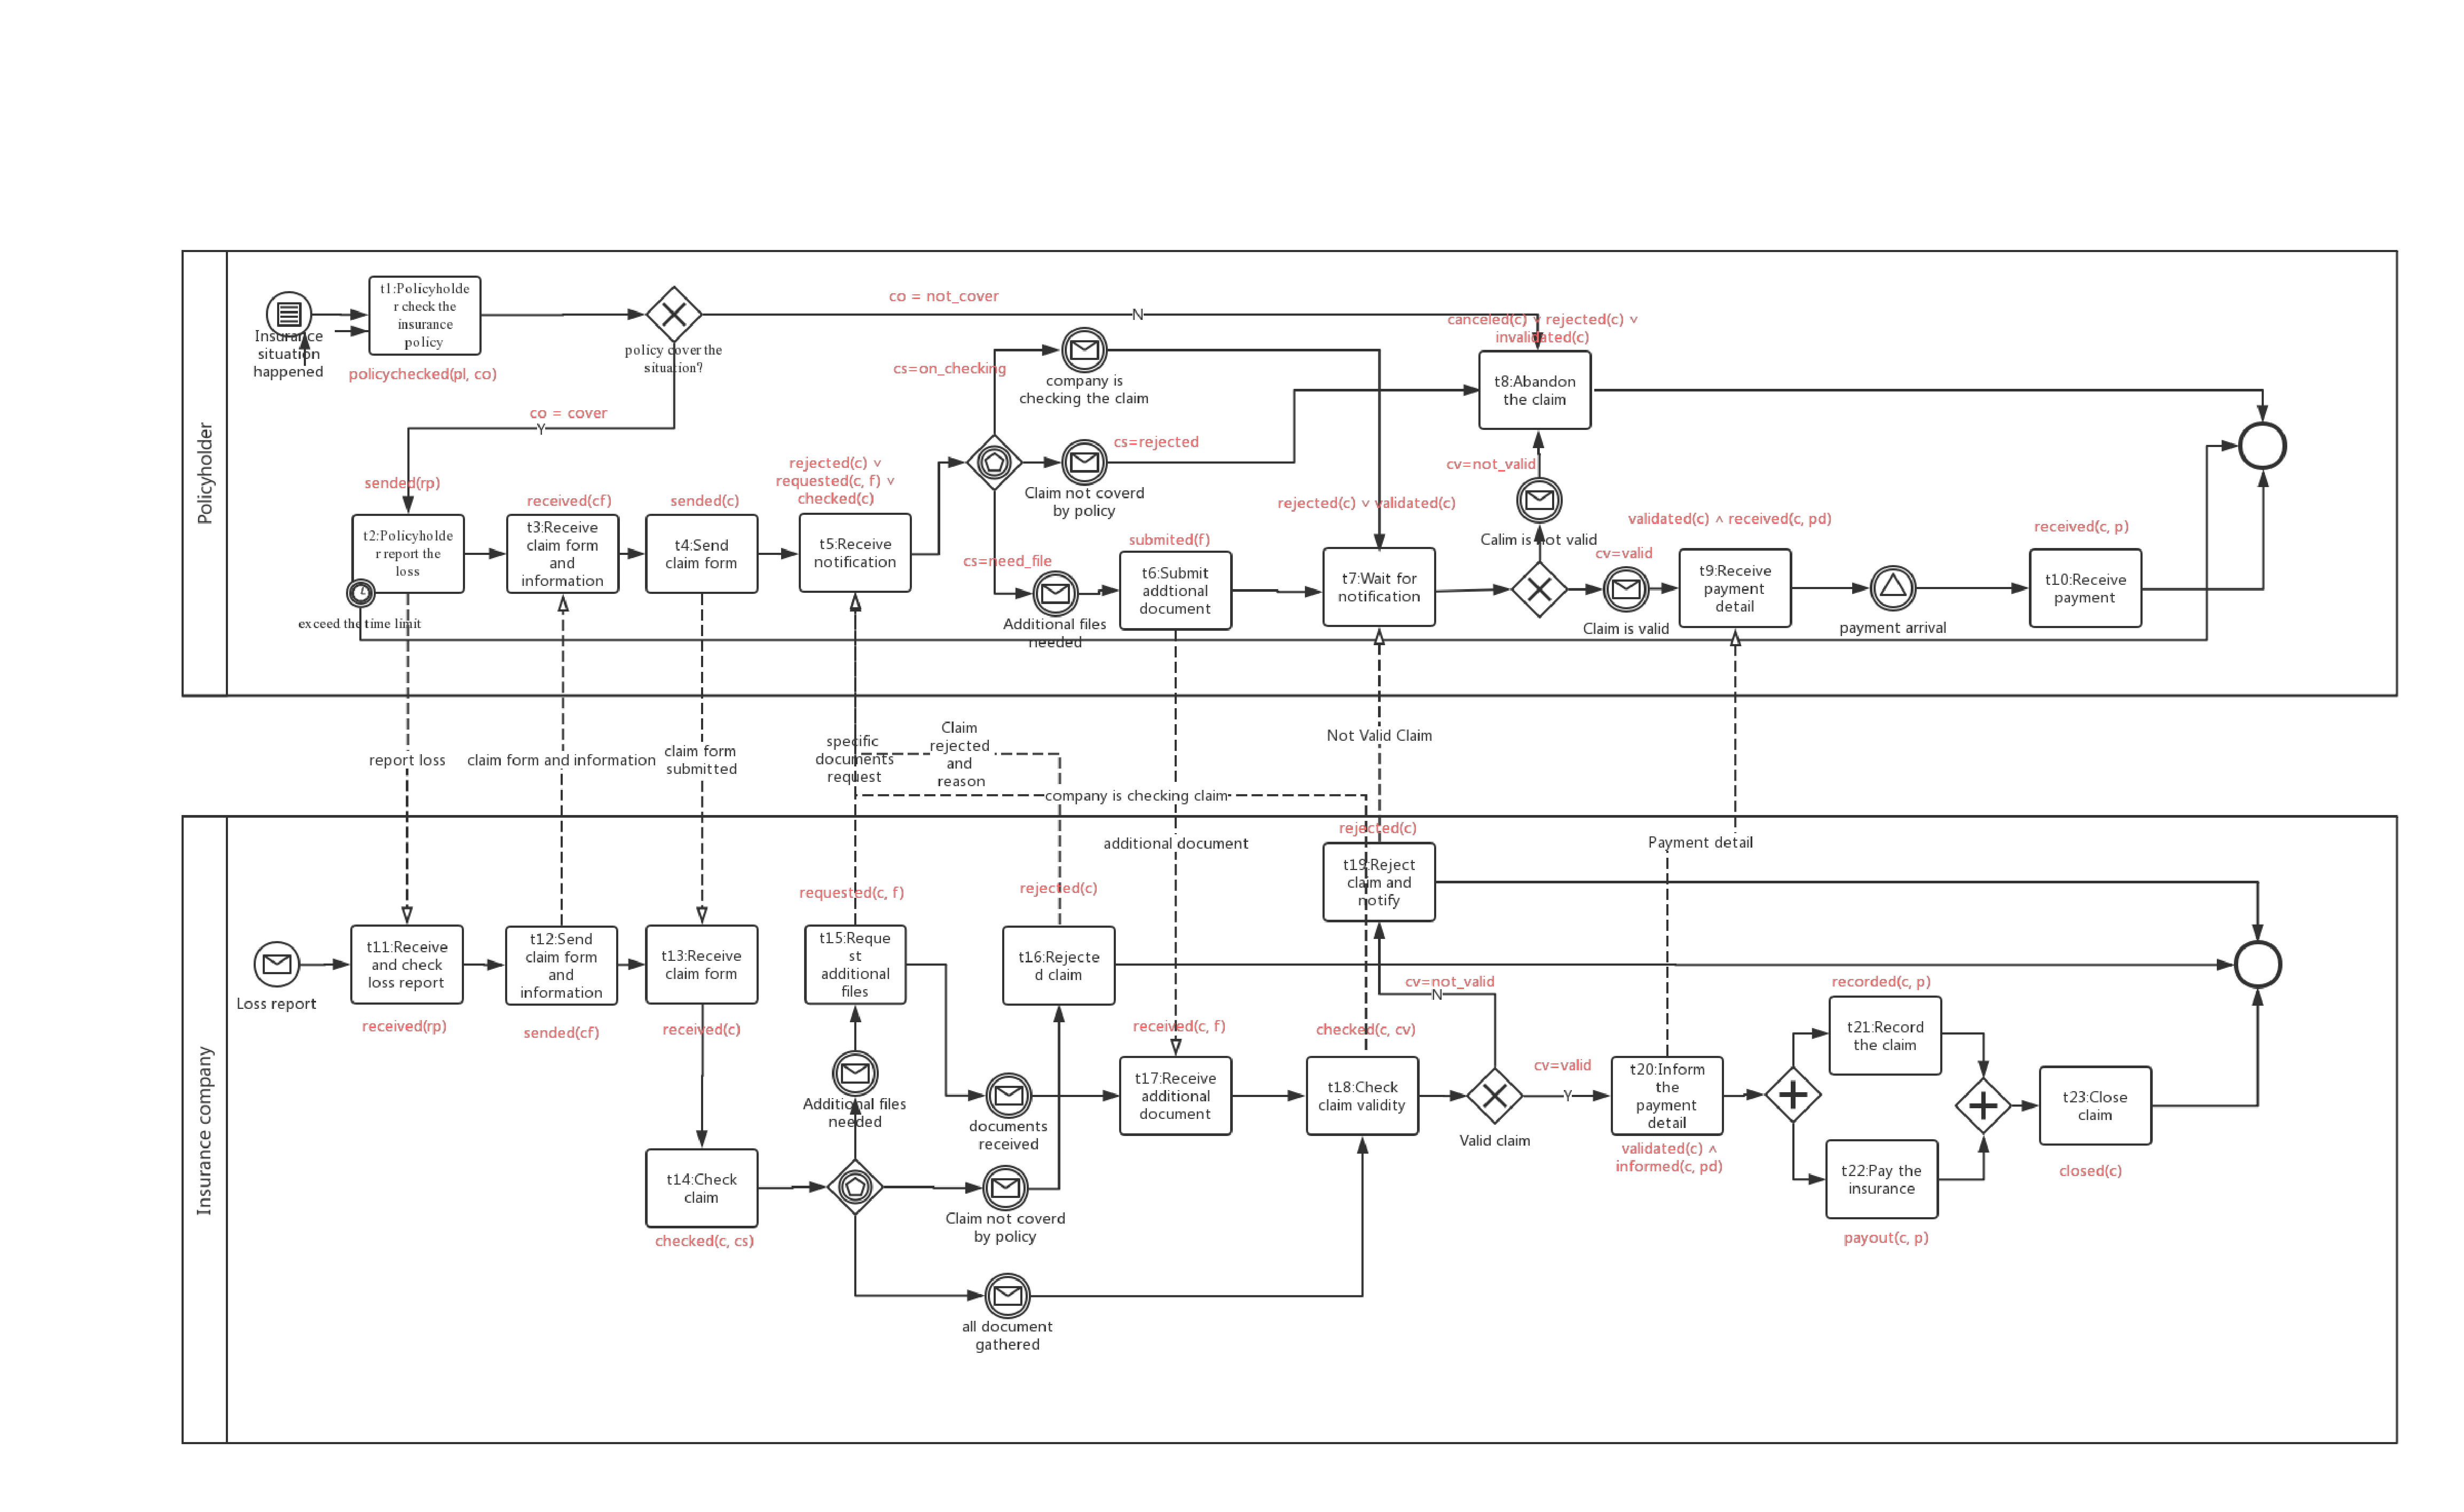
\includegraphics[width=1.0\textwidth]{BPMN} 
\caption{BPMN Model} 
\label{BPMN} 
\end{figure}

See figure \ref{BPMN}.



\subsection{Semantic Effect Annotation}
%-----------------------------------------------------------------------------------------------------------------------
% Please insert your designed BPMN model with Text Annotations on your BPMN model as a figure in this subsection.
%----------------------------------------------------------------------------------------------------------------------%

\begin{itemize}
\item[(a)]{Cumulative Effects of Tasks/Activities} \\
%----------------------------------------------------------------------------------------------------------------------
% Please provide the cumulative effects of tasks/activities as required.
%----------------------------------------------------------------------------------------------------------------------%
\textbf{pl=policy,co=ifcover,rp=report,cf=claimform,c=claim,f=file,p=payment}\\
t1=policychecked(po,co) \\
t2=sended(rp)\\
t3=received(cf)\\
t4=sended(c)\\
t5=rejected(c)$\vee$requested(c,f)$\vee$checked(c)\\
t6=submited(f)\\
t7=rejected(c)$\vee$checked(c)\\
t8=canceled(p)$\vee$rejected(c)$\vee$invalidated(c)\\
t9=validated(c)$\wedge$received(c,pd)\\                
t10=received(c,p)\\
t11=received(rp)\\
t12=sended(cf)\\
t13=received(c)\\
t14=checked(c,cs)\\
t15=requested(c,f)\\
t16=rejected(c)\\
t17=received(c,f)\\
t18=checked(c,cv)\\
t19=rejected(c)\\
t20=validated(c)$\vee$informed(c,pd)\\
t21=recorded(c,p)\\
t22=payout(c,p)\\
t23=closed(c)\\

$\forall c: policycover(c, not) \Leftrightarrow abandoned(c), \\ rejected(c) \Leftrightarrow closed(c), \\ invalidated(c) \Leftrightarrow abandoned(c) $
\\



\item[(b)]{Cumulative Effect Scenarios}
%----------------------------------------------------------------------------------------------------------------------
% Please provide the cumulative effect scenarios obtained at various points in the process as required.
%----------------------------------------------------------------------------------------------------------------------%
t2:scenerio(1):<t1,\{<t2>\}>\\
t8:scenario(1):<t1,\{<t8>\}>\\
t8:scenario(2):<t1,t2,t3,t4,t5,\{<t8>\}> \\
t8:scenario(2):<t1,t2,t3,t4,t5,t6,t7,\{<t8>\}> \\          
t10:scenario(1):<t1,t2,t3,t4,t5,t6,t7,t9,\{<t10>\}>\\
t16:scenerio(1):<t11,t12,t13,t14,\{<t16>\}>    \\
t19:scenerio(1):<t11,t12,t13,t14,t15,t17,t18,\{<t19>\}>\\
t19:scenerio(2):<t11,t12,t13,t14,t18,\{<t19>\}> \\
t23:scenerio(1):<t11,t12,t13,t14,t15,t17,t18,t20,{t21,t22},\{<t23>\}>\\
t23:scenerio(2):<t11,t12,t13,t14,t17,t18,t20,{t21,t22},\{<t23>\}>\\           

\end{itemize}

\section{PART TWO (3 MARKS)}
\subsection{Designed Petri Net}
%----------------------------------------------------------------------------------------------------------------------
% Please insert your designed Petri Net as a figure as required in this subsection.
%----------------------------------------------------------------------------------------------------------------------%

See figure \ref{petri}.

\begin{figure}
    \centering %图片居中
    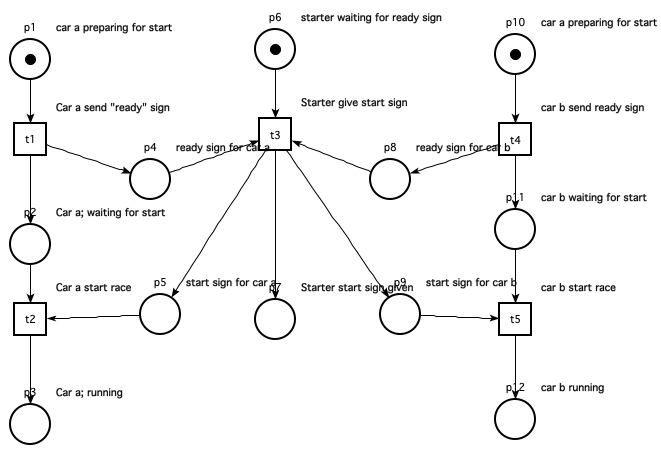
\includegraphics[width=1.0\textwidth]{petrinet} %插入图片,[]中设置图片大小,{}中是图片文件名
    \caption{Petri Net} %最终文档中希望显示的图片标题
    \label{petri} %用于文内引用的标签
\end{figure}





\subsection{Analysis on the Petri Net}
%----------------------------------------------------------------------------------------------------------------------
% Please give your analysis on your designed Petri Net by playing with a ``token game" in this subsection.
%----------------------------------------------------------------------------------------------------------------------%
First, place1 (car a preparing for start) has a token, when t1 transition fired (send ready sign) the token was send to place4 (p4 ready sign for car a) and place2 (p2 car a waiting for start). Place 6 is starter waiting for ready sign, when transmission3(t3 starter give start sign) fired, the token in p6 was copied and send to place 5,6,7. (start sign for car a,b and starter start sign given). in this time transition 2 was fired, car a turn to place 3(running). 

car b has the same situation.





\end{document}
